%%%%%%%%%%%%%%%%%%%%%%%%%%%%%%%%%%%%%%%%%%%%%%%%%%%%%%%%%%%%%%%%%%%%%%%%%%%%
% AGUtmpl.tex: this template file is for articles formatted with LaTeX2e,
% Modified March 2013
%
% This template includes commands and instructions
% given in the order necessary to produce a final output that will
% satisfy AGU requirements.
%
% PLEASE DO NOT USE YOUR OWN MACROS
% DO NOT USE \newcommand, \renewcommand, or \def.
%
% FOR FIGURES, DO NOT USE \psfrag or \subfigure.
%
%%%%%%%%%%%%%%%%%%%%%%%%%%%%%%%%%%%%%%%%%%%%%%%%%%%%%%%%%%%%%%%%%%%%%%%%%%%%
%
% All questions should be e-mailed to latex@agu.org.
%
%%%%%%%%%%%%%%%%%%%%%%%%%%%%%%%%%%%%%%%%%%%%%%%%%%%%%%%%%%%%%%%%%%%%%%%%%%%%
%
% Step 1: Set the \documentclass
%
% There are two options for article format: two column (default)
% and draft.
%
% PLEASE USE THE DRAFT OPTION TO SUBMIT YOUR PAPERS.
% The draft option produces double spaced output.
%
% Choose the journal abbreviation for the journal you are
% submitting to:

% jgrga JOURNAL OF GEOPHYSICAL RESEARCH
% gbc   GLOBAL BIOCHEMICAL CYCLES
% grl   GEOPHYSICAL RESEARCH LETTERS
% pal   PALEOCEANOGRAPHY
% ras   RADIO SCIENCE
% rog   REVIEWS OF GEOPHYSICS
% tec   TECTONICS
% wrr   WATER RESOURCES RESEARCH
% gc    GEOCHEMISTRY, GEOPHYSICS, GEOSYSTEMS
% sw    SPACE WEATHER
% ms    JAMES
% ef    EARTH'S FUTURE
%
%
%
% (If you are submitting to a jlineournal other than jgrga,
% substitute the initials of the journal for "jgrga" below.)



\documentclass[draft,ms]{AGUTeX}
\usepackage{graphicx}
\usepackage[modulo]{lineno}

% To create numbered lines:
%[pagewise] - Number continuously

% If you don't already have lineno.sty, you can download it from
% http://www.ctan.org/tex-archive/macros/latex/contrib/ednotes/
% (or search the internet for lineno.sty ctan), available at TeX Archive Network (CTAN).
% Take care that you always use the latest version.

% To activate the commands, uncomment \usepackage{lineno}
% and \linenumbers*[1]command, below:



\begin{document}

%  To add line numbers to lines with equations:
%  \begin{linenomath*}
%  \begin{equation}
%  \end{equation}
%  \end{linenomath*}
%%%%%%%%%%%%%%%%%%%%%%%%%%%%%%%%%%%%%%%%%%%%%%%%%%%%%%%%%%%%%%%%%%%%%%%%%
% Figures and Tables
%
%
% DO NOT USE \psfrag or \subfigure commands.
%
%  Figures and tables should be placed AT THE END OF THE ARTICLE,
%  after the references.
%
%  Uncomment the following command to include .eps files
%  (comment out this line for draft format):
%  \usepackage[dvips]{graphicx}
%
%  Uncomment the following command to allow illustrations to print
%   when using Draft:
%  \setkeys{Gin}{draft=false}
%
% Substitute one of the following for [dvips] above
% if you are using a different driver program and want to
% proof your illustrations on your machine:
%
% [xdvi], [dvipdf], [dvipsone], [dviwindo], [emtex], [dviwin],
% [pctexps],  [pctexwin],  [pctexhp],  [pctex32], [truetex], [tcidvi],
% [oztex], [textures]
%
% See how to enter figures and tables at the end of the article, after
% references.
%
%% ------------------------------------------------------------------------ %%
%
%  ENTER PREAMBLE
%
%% ------------------------------------------------------------------------ %%

% Author names in capital letters:
\authorrunninghead{Neale et al.}

% Shorter version of title entered in capital letters:
\titlerunninghead{E3SM Sub-Seasonal Tropical Variability}

%Corresponding author mailing address anE3SM_var_paper_wLENS_trmm_1deg_panel_PRECT.psd e-mail address:
%\authoraddr{Corresponding author: A. B. Smith,
%Department of Hydrology and Water Resources, University of
%Arizona, Harshbarger Building 11, Tucson, AZ 85721, USA.
%(a.b.smith@hwr.arizona.edu)}


%% ------------------------------------------------------------------------ %%
%
%  TITLE
%
%% ------------------------------------------------------------------------ %%


\title{Sub-Seasonal Tropical Variability in the DOE Earth \ Energy Exascale System Model (E3SM) version 1}
%
% e.g., \title{Terrestrial ring current:
% Origin, formation, and decay $\alpha\beta\Gamma\Delta$}
%

%% ------------------------------------------------------------------------ %%
%
%  AUTHORS AND AFFILIATIONS
%
%% ------------------------------------------------------------------------ %%


%Use \author{\altaffilmark{}} and \altaffiltext{}

% \altaffilmark will produce footnote;
% matching \altaffiltext will appear at bottom of page.
\authors{R. B. Neale,\altaffilmark{1}
 C. Hannay,\altaffilmark{1} S. Xie\altaffilmark{2} W. Lin\altaffilmark{2},
 J. Bacmeister\altaffilmark{1}}

\altaffiltext{1}{National Center for Atmospheric Research (NCAR), Boulder, Colorado, USA.}
\altaffiltext{2}{Lawrence Livermore National Laboratory, Berkeley, California, USA}

% \authors{A. B. Smith,\altaffilmark{1}
% Eric Brown,\altaffilmark{1,2} Rick Williams,\altaffilmark{3}
% John B. McDougall\altaffilmark{4}, and S. Visconti\altaffilmark{5}}

%\altaffiltext{1}{Department of Hydrology and Water Resources,
%University of Arizona, Tucson, Arizona, USA.}

%\altaffiltext{2}{Department of Geography, Ohio State University,
%Columbus, Ohio, USA.}

%\altaffiltext{3}{Department of Space Sciences, University of
%Michigan, Ann Arbor, Michigan, USA.}

%\altaffiltext{4}{Division of Hydrologic Sciences, Desert Research
%Institute, Reno, Nevada, USA.}

%\altaffiltext{5}{Dipartimento di Idraulica, Trasporti ed
%Infrastrutture Civili, Politecnico di Torino, Turin, Italy.}

%% ------------------------------------------------------------------------ %%
%
%  ABSTRACT
%
%% ------------------------------------------------------------------------ %%

% >> Do NOT include any \begin...\end commands within
% >> the body of the abstract.
\linenumbers
\modulolinenumbers[1]

\begin{abstract}

The Department of Energy (DOE) Energy Earth Exascale System Model (E3SM) is a state of the art modeling system with one particular focus on the global water cycle. As part of this assessment we present an examination of the variability in the tropics in the E3SM model on timescales important for impactful weather and its prediction beyond that of traditional forecasting timescales, namely sub-seasonal timescales. The model exhibits significant improvements in precipitation and cloud radiative forcing, indicative of an improved representation of convective variability. For precipitation there is close agreement with observations, but for OLR variance is still too weak. Organized modes of variability are a key component to many tropical seasonal and interannual variations, e.g., Monsoons, ENSO and the ITCZ. E3SM performs particularly well with a much improved Madden Julian Oscillation (MJO) compared to the baseline CESM1 model, but it does weaken higher frequency Kelvin Wave modes with too fast waves speeds. Although the MJO strength improved in frequency it is too regular with events occurring almost every Winter/Spring,. Furthermore 

The geographical locations for the coherent propagation of cloud/precipitation and dynamical signals as part of the MJO are dramatically improved such its influence can now be seen out of the Indian Oean and into the West Pacific. As to the  reasons for the changes and improvements to variability it i s clear that convection modifications, vertical resolution and coupling all have a role to play. Finally, the extra-seasonal impact of these intra-seasonal improvements can be illustrated by a much more significant relationship between ENSO activity and MJO strength. 


\end{abstract}

%% ------------------------------------------------------------------------ %%
%
%  BEGIN ARTICLE
%
%% ------------------------------------------------------------------------ %%

% The body of the article must start with a \begin{article} command
%
% \end{article} must follow the references section, before the figures
%  and tables.

\begin{article}

%% ------------------------------------------------------------------------ %%
%
%  TEXT
%
%% ------------------------------------------------------------------------ %%

\section{Introduction}
Climate model development has historically focused on seasonal and longer timescales to determine performance (REF, CAM4,GFDL4). However, variability on shorter sub-seasonal/intraseasonal timescales (days to weeks) is increasingly recognized as an equally important component of the climate system, essential for climate performance on longer timescales (REF). In the tropics sub-seasonal variability explains a significant portion of the total variance in precipitation and clouds, and is often key to the extreme events that can occur. 

A significant portion of the sub-seasonal variability is associated with equatorially trapped, convectively coupled waves. Many of these wave modes mimic those of a shallow water system and can be categorized according to dispersion and equivalent depth properties as Kelvin, Inertio-Gravity and Rossby waves among others. While these modes play a significant role in tropical variability, the propagating mode that dominates on sub-seasonal is the Madden Julian Oscillation (MJO). The propagating mode is somewhat different, in that it does not conform to any dispersion/equivalent depth behavior of shallow water system. Instead, previous work has proposed a number of theories for the MJO including Equatorial wave CISK, evaporation-wind feedback and moisture theory among others. Furthermore, there are uncertainties as to the role of the coupled system in supporting the MJO, but Sea Surface Temperature (SST) anomalies maybe be setting the slow speed of the convective envelope, particularly in the West Pacific warm pool    

There is also interaction among the sub-seasonal modes of variability, with implications for extreme event occurrence. For example over the Maritime Continent the diurnal cycle of precipitation dominates, but as intraseasonal MJO activity periodically traverses the region the diurnal mode becomes significantly suppressed (REF). Seasonal monsoon activity is also regulated by active break cycles, part of which is the northward propagating component of the MJO into the Indian sub-continent, causing breaks in the mostly regular seasonal monsoon activity, as well as being able to skew probablities of rainfall in the Australian Northern Monsoon region. Also the local influence of the MJO in spawning or suppressing tropical cyclone activity is well documented over the major cyclone basins. 

The up-scale role of sub-seasonal tropical variability within and exogenous to the tropics is increasingly being recognized, as important to the simulation in climate models, but also to the extension of skill in global forecast models. The MJO has a timescale and persistence that has been shown to more positively impact traditional forecast skill measures, when the host model is able to maintain an initial states that contain an MJO. This is possible as the MJO generates significantly large and extensive heating and associated divergence anomalies that can force planetary Rossby waves that impact the extra-tropical environment, particularly over the North Pacific and North America.


In Global Climate Models (GCMs), their performance at simulating sub-seasonal variability has been demonstrably poorer than other aspects of the tropical on longer timescales such as for ENSO and the Inter-tropical Convergence Zone (ITCZ). In particular modeling centers have struggled to consistently simulate an skillful diurnal cycle of precipitation over land, the PDF of precipitation and an acceptable MJO. Common biases include a peak in the diurnal cycle of rainfall that is too early in the day, a PDF of precipitation that has too few dry days, excessive drizzle and too few intense rainfall days, and an MJO that is either absent or propagates with a too rapid phase speed. Biases in these and other phenomena will clearly have up-scale implications for the seasonal and mean climate in GCMs.

=Basic state


Understanding the shortcomings of climate models in simulating sub-seasonal variability and determining what is needed to improve their skill has along been a challenge. Central to the processes that determine sub-seasonal variability in the tropics is predominantly atmospheric convection. Indeed, missing processes and sensitivities in the representation of deep convection are thought responsible for shortcomings in the simulation of variability. A major problem with the parameterization of deep convection has been it's over-sensitivity to surface properties, particularly over land, and it's low sensitivity to tropospheric dry regions. These characteristics had a direct impact on the common sub-seasonal variability model biases mentioned previously: the diurnal cycle is too responsive to surface forcings and destabilizes too early, the PDF of precipitation is not restricted by a dry troposphere and has too few no-rainfall days, and the MJO convection consumes convective energy too readily and is unable to slow build convective energy as part of a moisture mode. Recent enhancements to moisture sensitivity in convective parameterizations in different modeling, primarily through entrainment augmentation has led to demonstrable improvements to many of these sub-seasonal variability phenomena. As with many other phenomena, increases in resolution are proposed to help sub-seaonal variability biases. Significant improvements to the MJO have been seen in response to increass in vertical resolution \citep{Inness2001}, and these can be attributable to better resolved stable layers, mimicking a similar enhanced sensitivity to humidity as is seen with deep convection changes. 

We aim to the primarily document the characteristics of sub-seasonal variability in the Earth Energy Exascale System Model (E3SM) v1 and contrast behavior with the NCAR Community Earth System Model (CESM) v1., which was the starting point for E3SM development. Significant changes have been made to the representation of processes and model configuration that will be relevant to tropical sub-seasonal variability, so there is a reasonable expectation that changes will have occurred during the development process.


We describe model configurations and simulations in Chapter 1, and present the baseline sub-seasonal variability characteristics in Chapter 3. Chapter 4 will outline the behavior of equatorially trapped models of variability with a more focused analysis of the MJO in Chapter 5. An analysis of the diurnal cycle variability is presented in Chapter 6. To contrast both the role of atmosphere-ocean coupling and physical parameterization changes in E3SM, we examine sensitivity experiments in Chapter 6. Discussion and conclusions of model performance sill be summarized in Chapter 7.



\section{The Earth Energy Exascale Model (E3SM)}
The Department of energy (DOE) E3SM is a recently released fully coupled climate model development for research where one of the focus areas is the global water cycle. The model was originally based upon the Community Earth System Model (CESM1, REF), but it has been subject to multiple modifications since then.
\subsection{Atmosphere}
The first major modifications that were made were resolution and dynamical core changes. The finite volume dynamical core in CESM1 (REF,Lin Rood) was replaced by the spectral element (SE) core (REF). Although, the nominal horizontal resolution remains at 1\deg the numerics are performed on an unstructured cubed sphere grid with high-order advection. The 30-level configuration in CESM1 has been expanded to include 72 levels in the vertical, an approximate doubling of levels in the troposphere and lower stratosphere. This additionally includes a thin 20-m surface layer and an lifting of the model lid from around 40 km to 65 km, which now extends to the lower stratosphere.

The most relevant E3SM Atmosphere Model (EAM) changes to the water cycle are related to the moist processes. Although deep convection parameterization is essentially the same as in CESM there are some minor, yet potentially impactful modifications. 



\subsection{Surface Components}





\section{Winter-time mean and variability}
Properties of sub-seasonal tropical climate variability can be crucially dependent on the basic state of the model (REF). This can be seen for both unfiltered variability and for variability filtered in time an space. The mean and standard deviation of daily precipitation (Fig. \ref{f_mean_var_PRECT_DJF}) for northern hemisphere winter (DJF), the dominant season for tropical wave variability, show significant pattern changes in E3SM. West Pacific precipitation increases due to the moderation of equatorial cool SST biases and this is co-located with an increase in the standard deviation of precipitation, indicating the potential for significantly greater sub-seasonal variability. Conversely, a much drier South Pacific Convergence Zone (SPCZ) is coincident with a decrease in the precipitation variability bias. This is a crucial region for the DJF MJO as it can often have a propagating component that traverses down the SPCA when moving out of the West Pacific. 

A similar picture emerges from lower tropospheric zonal-wind, an important indicator of convectively coupled activity. In Fig. \ref{f_mean_var_U850_DJF} we see somewhat of a degradation of the mean wind field moving towards the mid-latitudes, but also in the deep tropics. Most crucially in the Indo-Pacific the pattern of the biases reverse from CESM1 with westerly bias in the Indian Ocean and easterly biases in the West Pacific being replaced by similar magnitude biases but of the opposite sign. These changes may be minor, but they occur in one of the limited number of regions in the tropics where the near-surface zonal wind is westerly. For eastward propagating disturbance westerly winds are key for surface flux enhancement mechanisms such as Wind Induced Surface Heat Exchange (WISHE)(REF) and the switch to westerly bias in the west Pacific could be enough to make the mean DJF field westerly in E3SM. Coincident with these changes there is a large increase in the standard deviation of 850-hPa wind, which may well be indicative of variability due to more consistent east propagating systems through the Indonesia/West Pacific regions, as we will see in later sections. Principally, the presence of Westerly Wind Bursts (WWB) may be responsible.

-Variance for seasons (PRECT,OLR,U850,CHI200?)

Focusing on particular Indo-Pacific regions, PDFs of daily precipitation variability (Fig. \ref{f_pdf_PRECT}) show significant changes in E3SM compared to CESM1, that do not necessarily reflect the overall regional increases in variability. Moving from West to East through the Indo-Pacific region both the PDF of precipitation grid-points and the PDF of rate contributions to the mean reflect changes in the model physics. Over India the overestimate of average precipitation is reduced significantly in E3SM. This is associated with an improvement in the excessive high precipitation rates, but there is also a shift from the lowest to the mid-range precipitation rates. The pattern shift is largely repeated over Indonesian land regions, but with a smaller change at the larger precipitation rates. This probably reflects the more maritime nature of the island climates. These changes do however exist exist in the presence of an increased negative mean bias. In the West Pacific region, key to mature propagating MJOs, precipitation mean biases increases significantly from CESM1. In parallel the PDF shape changes are the most marked of all focus regions. The frequency of moderate rates of 2-10 mm/day and 10-20 mm/day in particular are reduced significantly and represent an improvement. These low rate decreases in occurrence are offset by an improved increase in frequency beyond about 300 mm/day. To a large extent these distribution shifts are not seen in the East Pacific, which may in part reflect the very different underlying climate and in particular the nature of the propagating disturbances.

A documented problem with CESM1 and many other climate models is too frequently occurring weak precipitation rates (REF). This behavior can be seen across all regions where effectively zero precipitation rates (0-0.01 mm/day) occur infrequently compared to observations. Non-precipitating periods are key to the convective recharge behavior in the tropics. The most likely explanation for this improved behavior is the tighter restraint applied to the system (capeten change) where individual stable layers in a column are able to restrict deep convection and precipitation during dryer and more stable conditions. This then allows this recharge to occur, likely leading to improved propagating wave characteristics seen in E3SM.

Overall the unfiltered variance in precipitation and dynamical fields sees an increase in E3SM, which may, to a certain extent, be explained by shifts in the PDFs of precipitation rate, particularly due to an increase in high precipitation rates. Filtering, for the sub-seasonal time frame of reference (20-100 days) an increases in variance in E3SM is retained. Averaged through the Indo-Pacific region.


\section{Sub-seasonal Organization}
-Total tropical variability (KF, PRECT/OMEGA500/U850/FLUT/CHI200?)
-kf extraction hovmoeller plots
-Lag-correlation/covariance plots.
-Composite patterns

Although sub-seasonal variability had on the whole appeared to have increased this does not necessarily speak to the nature of the variability as it related to propagating phenomena. Figure shows a decomposition of precipitation variability into wavenumber-frequency power spectrum following REF -WK. They are raw spectrum showing predominantly a red spectral behavior in precipitation whereby the greatest power exist in the longest wavelength and period disturbances. There are deviations from pure red behavior where the maximum power is at wavenumbers 1-4, and periods of around 30 days and longer. Furthermore, the deviations from red behavior occur depending on the westward or eastward propagating directions.

Whereas observations of precipitation for TRMM and GPCP are largely in agreement for mean distributions, the 2D spectral behavior differs significantly. At the reddest part of the spectrum differences are small, but for smaller scale, higher frequency differences.

The tropics are observed to support a number of equatorially trapped disturbance that exhibit simpler wave-like dispersion characteristics. Taking the full symmetric spectrally decomposed field from Fig. \ref{f_kf_sym_PREC} and dividing by a smoothed total field, we are able to reveal regions of above-red power in the precipitation propagating field.   



\section{Diurnal variability}
-Diurnal cycle phase (semi-diurnal)
+PRECT/PRECL/PRECC maybe
-OMEGA500/CLOUD

On sub-daily timescales the dominant forcing mode of variability in the tropics is the diurnal cycle, and the pattern of rainfall in response to surface forcing over land, land-sea contrasts and cloud-top cooling and stability changes over the ocean. The correct simulation of the diurnal cycle of (REF) precipitation has been a major challenge for climate models (REF), largely due to the generally course horizontal grid resolutions (~100 km) and related need to parameterize the effects of deep convection. 




\section {Sensitivity Experiments}
To determine the role of different developments that are included as part of the E3SM Atmosphere Model (EAMv1). 

\section{Ocean Atmosphere Coupling}
\section{Extra-seasonal Variability}
\section{Conclusions}
The E3SM Atmosphere Model (EAM) is a state of the art atmosphere modeling system and represents a significant contribution to earth system research. Modifications have been made both to the representation of physical processes, but also the resolution and dynamical framework. These changes have significant impacts on the simulation of atmosphere phenomena including for mean climate and variability on a range of time and space scales.

%%% End of body of article:

%%%%%%%%%%%%%%%%%%%%%%%%%%%%%%%%
%% Optional Appendix goes here
%
% \appendix resets counters and redefines section heads
% but doesn't print anything.
% After typing \appendix
%
%\section{Here Is Appendix Title}
% will show
% Appendix A: Here Is Appendix Title
%
%%%%%%%%%%%%%%%%%%%%%%%%%%%%%%%%%%%%%%%%%%%%%%%%%%%%%%%%%%%%%%%%
%
% Optional Glossary or Notation section, goes here
%
%%%%%%%%%%%%%%
% Glossary is only allowed in Reviews of Geophysics
% \section*{Glossary}
% \paragraph{Term}
% Term Definition here
%
%%%%%%%%%%%%%%
% Notation -- End each entry with a period.
% \begin{notation}
% Term & definition.\\
% Second term & second definition.\\
% \end{notation}
%%%%%%%%%%%%%%%%%%%%%%%%%%%%%%%%%%%%%%%%%%%%%%%%%%%%%%%%%%%%%%%%
%
%  ACKNOWLEDGMENTS

\begin{acknowledgments}
The National Center for Atmospheric Research is sponsored by the National Science Foundation.
\end{acknowledgments}



%% ------------------------------------------------------------------------ %%
%%  REFERENCE LIST AND TEXT CITATIONS
%
% Either type in your references using
%\begin{thebibliography}{}
% \bibitem{}
% Text
% \end{thebibliography}
%
% Or,
%
% If you use BiBTeX for your references, please use the agufull08.bst file (available at % ftp://ftp.agu.org/journals/latex/journals/Manuscript-Preparation/) to produce your .bbl
% file and copy the contents into your paper here.
%
% Follow these steps:
%
% 2. Make sure the bibliography style appears as
%\ifthenelse{\boolean{dc}}
%{}
%{\clearpage}

\bibliographystyle{BibTeX/agufull08}.
\bibliography{BibTeX/references}


%% FIGURES %%

\begin{figure}[t]
  \begin{center}
    \noindent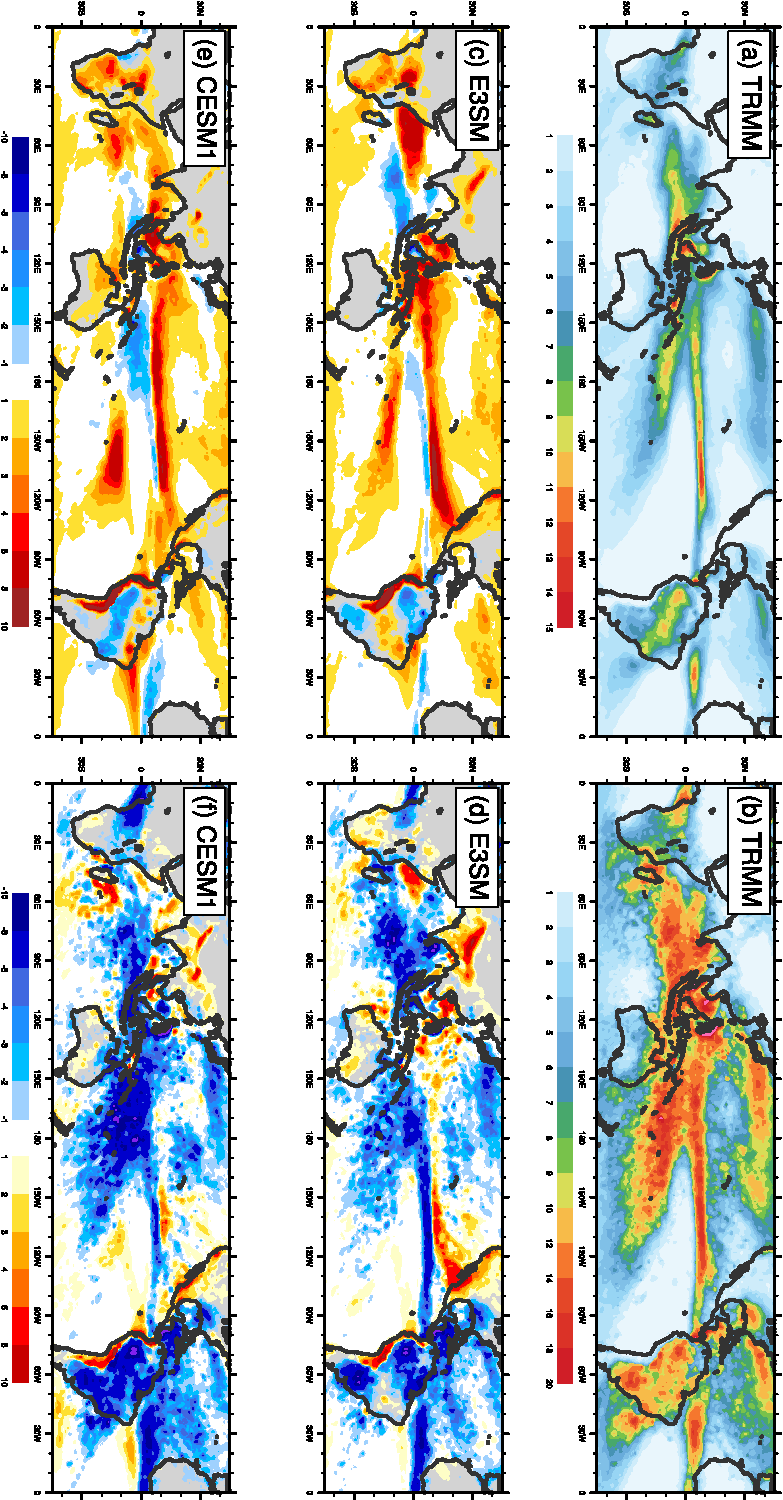
\includegraphics[width=0.5\textwidth,angle=90.]{./figs/f_mean_var_PRECT_DJF.pdf}
  \end{center}
  \caption{Observed TRMM Precipitation (1999-2013) for (a) mean and (b) standard deviation of daily amounts in mm/day. Difference from observations for E3SM (c) mean, (d) standard deviation and for CESM1 (e) mean and (f) standard deviation. Model average periods are for 15 years.} 
\label{f_mean_var_PRECT_DJF}
\end{figure}

\begin{figure}[t]
  \begin{center}
    \noindent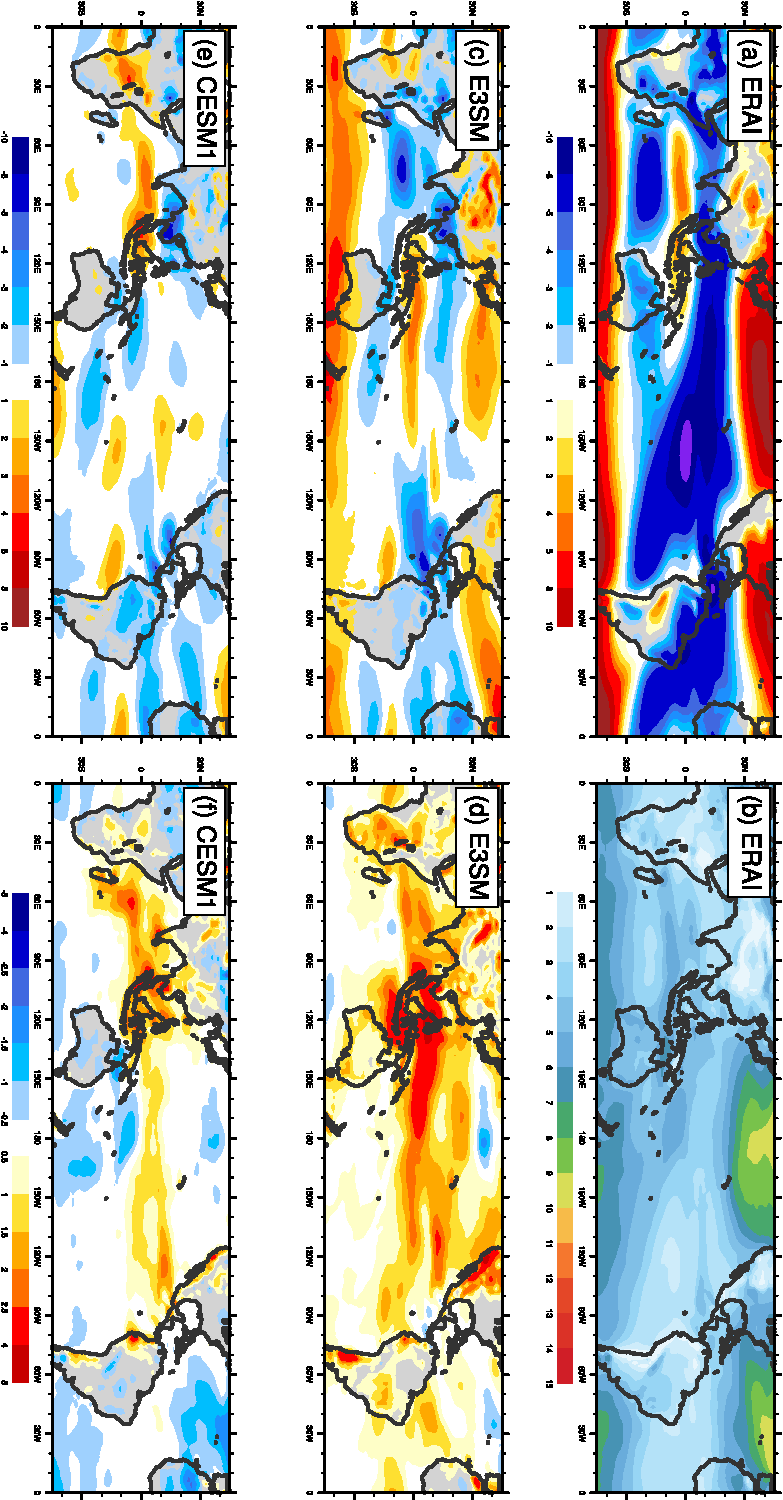
\includegraphics[width=0.5\textwidth,angle=90.]{./figs/f_mean_var_U850_DJF.pdf}
  \end{center}
  \caption{Observed ERA-interim 850-hPa zonal wind (1999-2013) for (a) mean and (b) standard deviation of daily amounts in mm/day. Difference from observations for E3SM (c) mean, (d) standard deviation and for CESM1 (e) mean and (f) standard deviation. Model average periods are for 15 years} 
\label{f_mean_var_U850_DJF}
\end{figure}



\begin{figure}[t]
  \begin{center}
    \noindent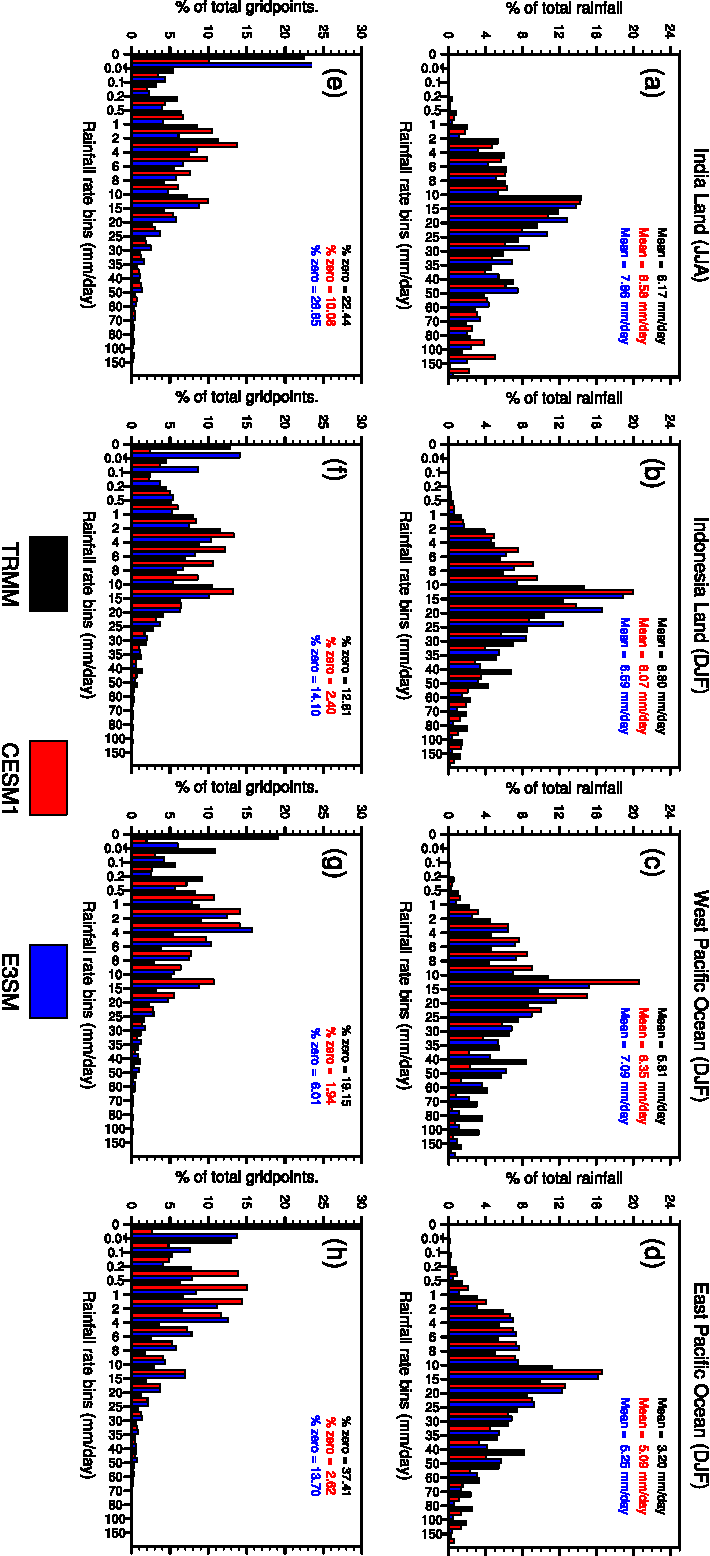
\includegraphics[width=0.5\textwidth,angle=90.]{./figs/f_pdf_PRECT.pdf}
  \end{center}
  \caption{Seasonal probability distributions of daily precipitation rate (mm/day) for 15 years over Indo-Pacific regions: India Land (region), Indonesia Land (region), West Pacific Ocean (region) and East Pacific Ocean (region). (a) through (d) is the percentage of total rainfall that each bin contributes. (e) through (h) is the percentage of the total number samples contributing to that rainfall rate. TRMM observations are interpolated to a 1 degree grid coincident with the model grid.} 
\label{f_pdf_PRECT}
\end{figure}

\begin{figure}[t]
  \begin{center}
    \noindent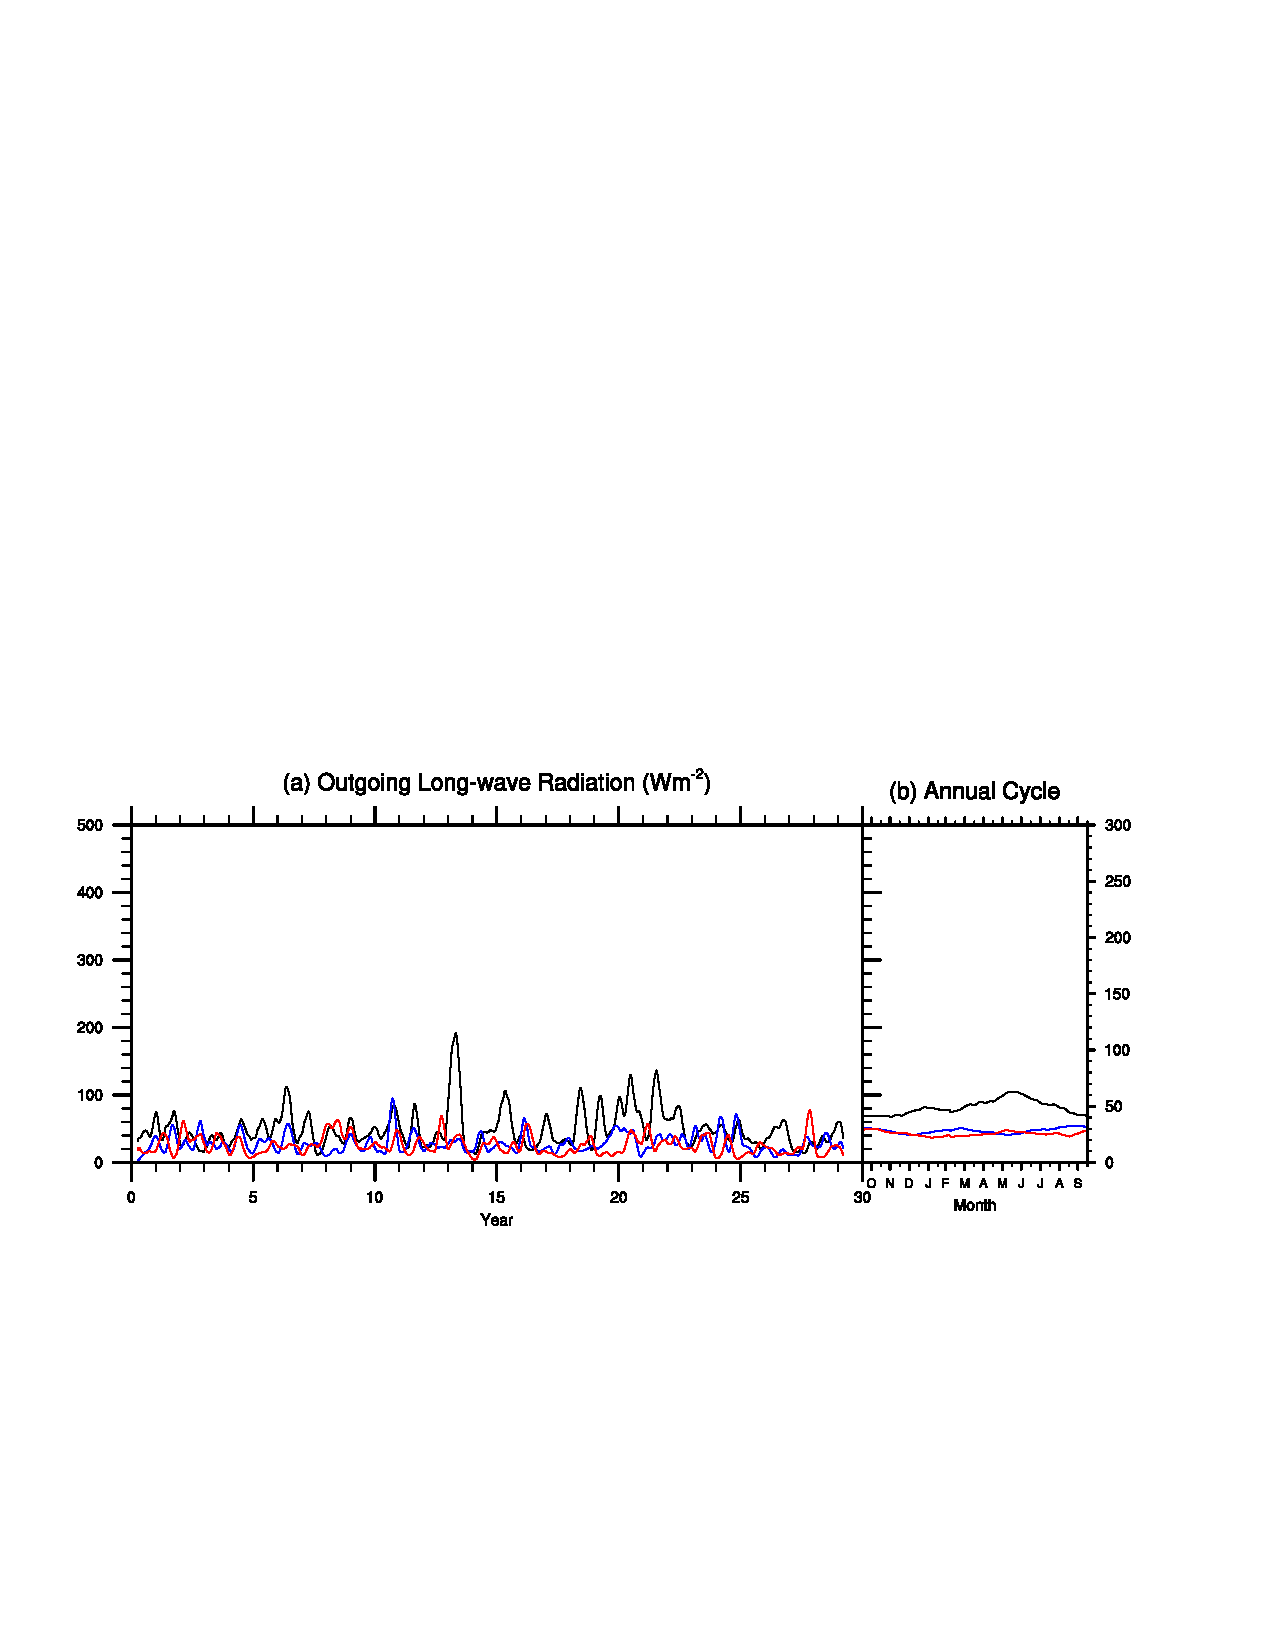
\includegraphics[width=1.1\textwidth,angle=0.]{./figs/f_bpass.pdf}
  \end{center}
  \caption{Band pass (20-100 days) filtered daily outgoing long-wave radiation Wm$^{-2}$} 
\label{f_bpass}
\end{figure}

\begin{figure}[t]
  \begin{center}
    \noindent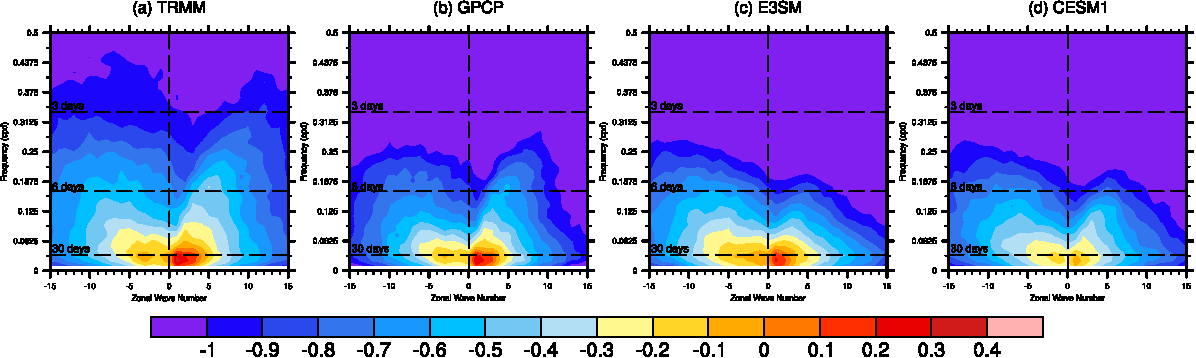
\includegraphics[width=1.1\textwidth,angle=0.]{./figs/f_kf_sym_PRECT.pdf}
  \end{center}
  \caption{Wavenumber frequency power spectra for total precipitation [ln(mm/day)] (following WK REF) filtered for propagating disturbances symmetric about the equator (15\deg S-15\deg N)  (a) TRMM, (b) GPCP, observations and historical simulations (1979-1986) (C) E3SM  and (d) CESM1.} 
\label{f_kf_sym_PRECT}
\end{figure}

\begin{figure}[t]
  \begin{center}
    \noindent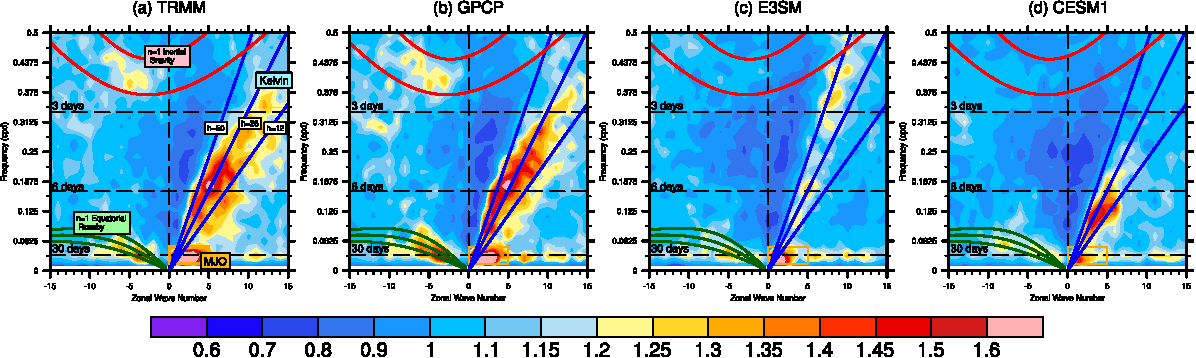
\includegraphics[width=1.1\textwidth,angle=0.]{./figs/f_kf_sym_ratio_PRECT.pdf}
  \end{center}
  \caption{Ratio of filtered wavenumber frequency power spectra for total precipitation, above smoothed (red) pseudo-background spectra of the same field (15\deg S-15\deg N),   (a) TRMM, (b) GPCP, observations and historical simulations (1979-1986) (C) E3SM  and (d) CESM1.} 
\label{f_kf_sym_ratio_PRECT}
\end{figure}


\begin{figure}[t]
  \begin{center}
    \noindent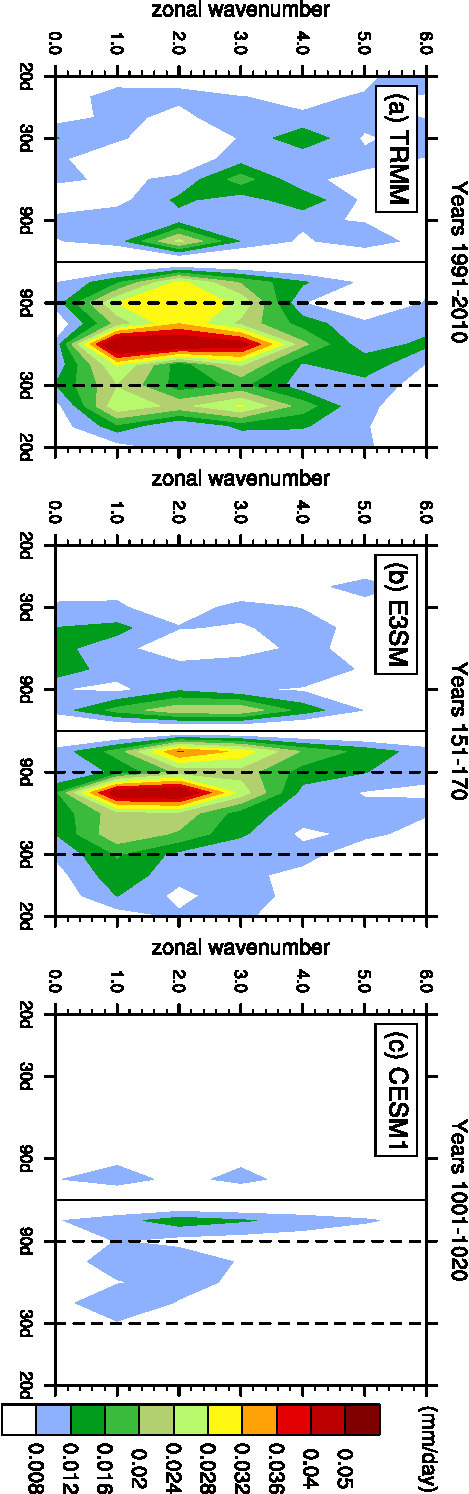
\includegraphics[width=0.3\textwidth,angle=90.]{./figs/f_mjo_spectra_PRECT_djf.pdf}
  \end{center}
  \caption{Mean var PRECT } 
\label{f_mjo_spectra_PRECT_djf}
\end{figure}

\begin{figure}[t]
  \begin{center}
    \noindent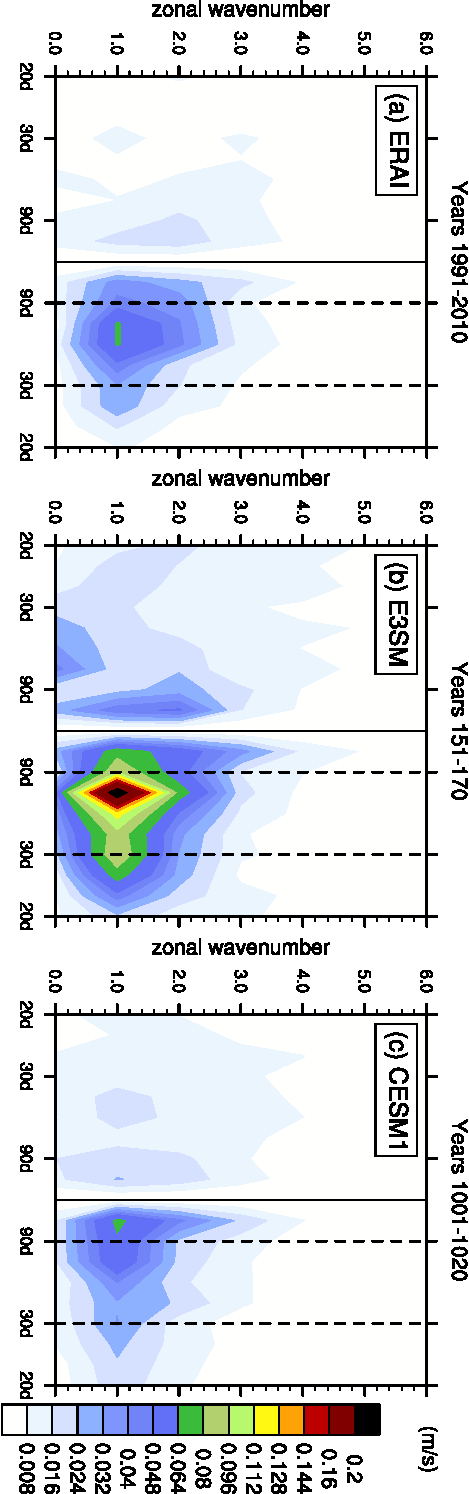
\includegraphics[width=0.3\textwidth,angle=90.]{./figs/f_mjo_spectra_U850_djf.pdf}
  \end{center}
  \caption{Mean var PRECT } 
\label{f_mjo_spectra_U850_djf}
\end{figure}

\begin{figure}[t]
  \begin{center}
    \noindent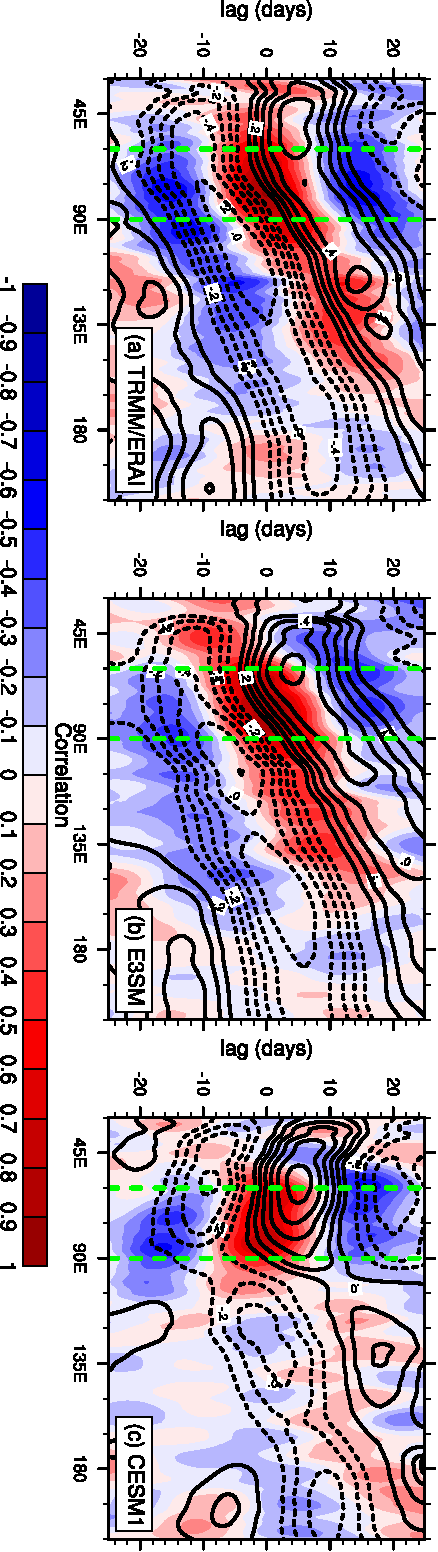
\includegraphics[width=0.3\textwidth,angle=90.]{./figs/f_lagcorr_djf.pdf}
  \end{center}
  \caption{Mean var PRECT (10N - 10S) } 
\label{f_lagcorr_djf}
\end{figure}

\begin{figure}[t]
  \begin{center}
    \noindent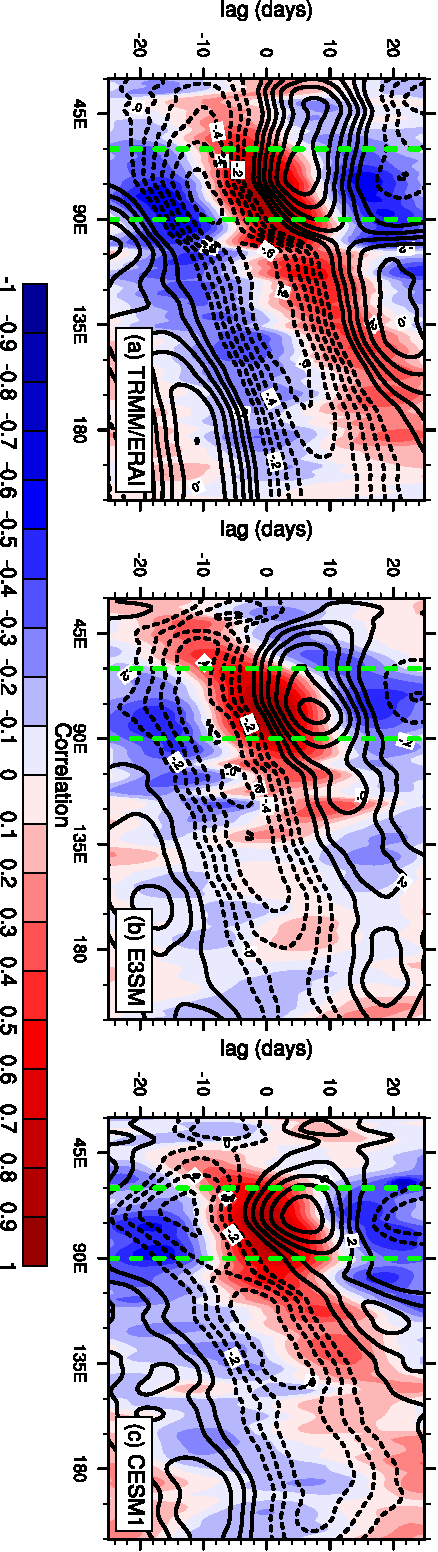
\includegraphics[width=0.3\textwidth,angle=90.]{./figs/f_lagcorr_jja.pdf}
  \end{center}
  \caption{Mean var PRECT (10N-10S) } 
\label{f_lagcorr_jja}
\end{figure}

\begin{figure}[t]
  \begin{center}
    \noindent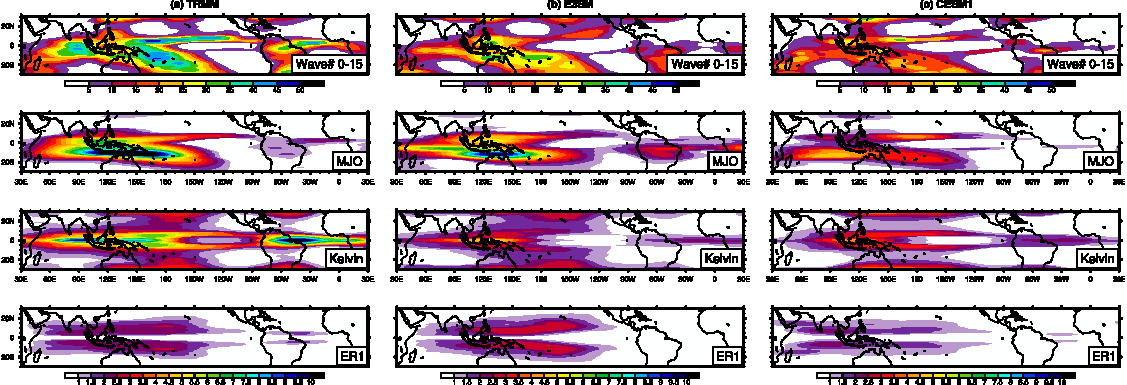
\includegraphics[width=1.1\textwidth,angle=0.]{./figs/f_wave_var_DJF_PRECT.pdf}
  \end{center}
  \caption{Regional variance of a inverse transformed daily precipitation field (mm/day)$^2$ after filtering for wavenumber frequency regions specific to wavenumbers -15 to +15 and for MJO, Kelvin and n=1 Rossby propagating modes of variability. Shown are (a) TRMM observations, with (b) E3SM and (c) CESM1 simulations≥} 
\label{f_wave_var_DJF_PRECT}
\end{figure}en filtering

\newpage

%Run BiBTeX on your LaTeX
% file.
%
% 3. Open the new .bbl file containing the reference list and
%   copy all the contents into your LaTeX file here.
%
% 4. Comment out the old \bibliographystyle and \bibliography commands.
%
% 5. Run LaTeX on your new file before submitting.
%
% AGU does not want a .bib or a .bbl file. Please copy in the contents of your .bbl file here.

%\begin{thebibliography}{}

%\providecommand{\natexlab}[1]{#1}
%\expandafter\ifx\csname urlstyle\endcsname\relax
%  \providecommand{\doi}[1]{doi:\discretionary{}{}{}#1}\else
%  \providecommand{\doi}{doi:\discretionary{}{}{}\begingroup
%  \urlstyle{rm}\Url}\fi
%
%\bibitem[{\textit{Atkinson and Sloan}(1991)}]{AtkinsonSloan}
%Atkinson, K., and I.~Sloan (1991), The numerical solution of first-kind
%  logarithmic-kernel integral equations on smooth open arcs, \textit{Math.
%  Comp.}, \textit{56}(193), 119--139.
%
%\bibitem[{\textit{Colton and Kress}(1983)}]{ColtonKress1}
%Colton, D., and R.~Kress (1983), \textit{Integral Equation Methods in
%  Scattering Theory}, John Wiley, New York.
%
%\bibitem[{\textit{Hsiao et~al.}(1991)\textit{Hsiao, Stephan, and
%  Wendland}}]{StephanHsiao}
%Hsiao, G.~C., E.~P. Stephan, and W.~L. Wendland (1991), On the {D}irichlet
%  problem in elasticity for a domain exterior to an arc, \textit{J. Comput.
%  Appl. Math.}, \textit{34}(1), 1--19.
%
%\bibitem[{\textit{Lu and Ando}(2012)}]{LuAndo}
%Lu, P., and M.~Ando (2012), Difference of scattering geometrical optics
%  components and line integrals of currents in modified edge representation,
%  \textit{Radio Sci.}, \textit{47},  RS3007, \doi{10.1029/2011RS004899}.

%\end{thebibliography}

%Reference citation examples:

%...as shown by \textit{Kilby} [2008].
%...as shown by {\textit  {Lewin}} [1976], {\textit  {Carson}} [1986], {\textit  {Bartholdy and Billi}} [2002], and {\textit  {Rinaldi}} [2003].
%...has been shown [\textit{Kilby et al.}, 2008].
%...has been shown [{\textit  {Lewin}}, 1976; {\textit  {Carson}}, 1986; {\textit  {Bartholdy and Billi}}, 2002; {\textit  {Rinaldi}}, 2003].
%...has been shown [e.g., {\textit  {Lewin}}, 1976; {\textit  {Carson}}, 1986; {\textit  {Bartholdy and Billi}}, 2002; {\textit  {Rinaldi}}, 2003].

%...as shown by \citet{jskilby}.
%...as shown by \citet{lewin76}, \citet{carson86}, \citet{bartoldy02}, and \citet{rinaldi03}.
%...has been shown \citep{jskilbye}.
%...has been shown \citep{lewin76,carson86,bartoldy02,rinaldi03}.
%...has been shown \citep [e.g.,][]{lewin76,carson86,bartoldy02,rinaldi03}.
%
% Please use ONLY \citet and \citep for reference citations.
% DO NOT use other cite commands (e.g., \cite, \citeyear, \nocite, \citealp, etc.).

%% ------------------------------------------------------------------------ %%
%
%  END ARTICLE
%
%% ------------------------------------------------------------------------ %%
\end{article}
%
%
%% Enter Figures and Tables here:
%
% DO NOT USE \psfrag or \subfigure commands.
%
% Figure captions go below the figure.
% Table titles go above tables; all other caption information
%  should be placed in footnotes below the table.
%
%----------------
% EXAMPLE FIGURE
%
% \begin{figure}
% \noindent\includegraphics[width=20pc]{samplefigure.eps}
% \caption{Caption text here}
% \label{figure_label}
% \end{figure}


%
% ---------------
% EXAMPLE TABLE
%
%\begin{table}
%\caption{Time of the Transition Between Phase 1 and Phase 2\tablenotemark{a}}
%\centering
%\begin{tabular}{l c}
%\hline
% Run  & Time (min)  \\
%\hline
%  $l1$  & 260   \\
%  $l2$  & 300   \\
%  $l3$  & 340   \\
%  $h1$  & 270   \\
%  $h2$  & 250   \\
%  $h3$  & 380   \\
%  $r1$  & 370   \\
%  $r2$  & 390   \\
%\hline
%\end{tabular}
%\tablenotetext{a}{Footnote text here.}
%\end{table}

% See below for how to make sideways figures or tables.

\end{document}

%%%%%%%%%%%%%%%%%%%%%%%%%%%%%%%%%%%%%%%%%%%%%%%%%%%%%%%%%%%%%%%

More Information and Advice:

%% ------------------------------------------------------------------------ %%
%
%  SECTION HEADS
%
%% ------------------------------------------------------------------------ %%

% Capitalize the first letter of each word (except for
% prepositions, conjunctions, and articles that are
% three or fewer letters).

% AGU follows standard outline style; therefore, there cannot be a section 1 without
% a section 2, or a section 2.3.1 without a section 2.3.2.
% Please make sure your section numbers are balanced.
% ---------------
% Level 1 head
%
% Use the \section{} command to identify level 1 heads;
% type the appropriate head wording between the curly
% brackets, as shown below.
%
%An example:
%\section{Level 1 Head: Introduction}
%
% ---------------
% Level 2 head
%
% Use the \subsection{} command to identify level 2 heads.
%An example:
%\subsection{Level 2 Head}
%
% ---------------
% Level 3 head
%
% Use the \subsubsection{} command to identify level 3 heads
%An example:
%\subsubsection{Level 3 Head}
%
%---------------
% Level 4 head
%
% Use the \subsubsubsection{} command to identify level 3 heads
% An example:
%\subsubsubsection{Level 4 Head} An example.
%
%% ------------------------------------------------------------------------ %%
%
%  IN-TEXT LISTS
%
%% ------------------------------------------------------------------------ %%
%
% Do not use bulleted lists; enumerated lists are okay.
% \begin{enumerate}
% \item
% \item
% \item
% \end{enumerate}
%
%% ------------------------------------------------------------------------ %%
%
%  EQUATIONS
%
%% ------------------------------------------------------------------------ %%

% Single-line equations are centered.
% Equation arrays will appear left-aligned.

Math coded inside display math mode \[ ...\]
 will not be numbered, e.g.,:
 \[ x^2=y^2 + z^2\]

 Math coded inside \begin{equation} and \end{equation} will
 be automatically numbered, e.g.,:
 \begin{equation}
 x^2=y^2 + z^2
 \end{equation}

% IF YOU HAVE MULTI-LINE EQUATIONS, PLEASE
% BREAK THE EQUATIONS INTO TWO OR MORE LINES
% OF SINGLE COLUMN WIDTH (20 pc, 8.3 cm)
% using double backslashes (\\).

% To create multiline equations, use the
% \begin{eqnarray} and \end{eqnarray} environment
% as demonstrated below.
\begin{eqnarray}
  x_{1} & = & (x - x_{0}) \cos \Theta \nonumber \\
        && + (y - y_{0}) \sin \Theta  \nonumber \\
  y_{1} & = & -(x - x_{0}) \sin \Theta \nonumber \\
        && + (y - y_{0}) \cos \Theta.
\end{eqnarray}

%If you don't want an equation number, use the star form:
%\begin{eqnarray*}...\end{eqnarray*}

% Break each line at a sign of operation
% (+, -, etc.) if possible, with the sign of operation
% on the new line.

% Indent second and subsequent lines to align with
% the first character following the equal sign on the
% first line.

% Use an \hspace{} command to insert horizontal space
% into your equation if necessary. Place an appropriate
% unit of measure between the curly braces, e.g.
% \hspace{1in}; you may have to experiment to achieve
% the correct amount of space.


%% ------------------------------------------------------------------------ %%
%
%  EQUATION NUMBERING: COUNTER
%
%% ------------------------------------------------------------------------ %%

% You may change equation numbering by resetting
% the equation counter or by explicitly numbering
% an equation.

% To explicitly number an equation, type \eqnum{}
% (with the desired number between the brackets)
% after the \begin{equation} or \begin{eqnarray}
% command.  The \eqnum{} command will affect only
% the equation it appears with; LaTeX will number
% any equations appearing later in the manuscript
% according to the equation counter.
%

% If you have a multiline equation that needs only
% one equation number, use a \nonumber command in
% front of the double backslashes (\\) as shown in
% the multiline equation above.

%% ------------------------------------------------------------------------ %%
%
%  SIDEWAYS FIGURE AND TABLE EXAMPLES
%
%% ------------------------------------------------------------------------ %%
%
% For tables and figures, add \usepackage{rotating} to the paper and add the rotating.sty file to the folder.
% AGU prefers the use of {sidewaystable} over {landscapetable} as it causes fewer problems.
%
% \begin{sidewaysfigure}
% \includegraphics[width=20pc]{samplefigure.eps}
% \caption{caption here}
% \label{label_here}
% \end{sidewaysfigure}
%
%
%
% \begin{sidewaystable}
% \caption{}
% \begin{tabular}
% Table layout here.
% \end{tabular}
% \end{sidewaystable}
%
%

